\documentclass[9pt]{osa-supplemental-document}
\setboolean{shortarticle}{false}
\setboolean{displaycopyright}{false}

\usepackage{float}
\usepackage{placeins}
\usepackage{array}

\renewcommand{\thesection}{S\arabic{section}}
\renewcommand{\thesubsection}{\thesection.\arabic{subsection}}
\newcommand{\suppheadingfont}{\fontfamily{phv}\selectfont}
\titleformat{\section}
  {\large\suppheadingfont\bfseries}
  {\thesection.}
  {0.5em}
  {\MakeUppercase{#1}}
  []
\titleformat{name=\section,numberless}
  {\large\suppheadingfont\bfseries}
  {}
  {0em}
  {\MakeUppercase{#1}}
  []
\titleformat{\subsection}
  {\suppheadingfont\bfseries}
  {\thesubsection.}
  {0.5em}
  {#1}
  []

\title{From Fog Chamber to Aircraft Window: Pixel-Registered Imaging and Synthetic Fine-Tuning Enable Cross-Domain Defogging: supplemental document}
\author{} %leave this blank
%% DO NOT ADD AUTHOR INFORMATION HERE; IT WILL BE ADDED DURING PRODUCTION

\begin{abstract}
\end{abstract}

\begin{document}
\maketitle

\section{Dataset Roles and Split Provenance}

Table~\ref{tabS:dataset_roles} summarizes dataset roles and split provenance. The fog-chamber task is the only cross-architecture benchmark. The synthetic-fine-tuned, mixed O-HAZE+NH-HAZE, and NTIRE nighttime haze models are NAFNet fine-tuning regimes started from the same fog-chamber model. The synthetic-fine-tuned model is evaluated as direct transfer on fog-machine, aircraft-window, and public paired-haze examples; the public paired-haze and NTIRE task-specific models use supervised fine-tuning on their own training splits.

The public reproduction package is split across GitHub and Kaggle. Code and lightweight result tables are released at \url{https://github.com/theMenonlab/defogging}. Trained NAFNet model weights are released at \url{https://www.kaggle.com/models/alingold/fog-removal}. The fog-chamber dataset is released at \url{https://www.kaggle.com/datasets/alingold/fog-chamber}. The Mapillary Vistas source images for synthetic fine-tuning are available at \url{https://www.kaggle.com/datasets/kaggleprollc/mapillary-vistas-image-data-collection}, and the source image archive used for display capture is available at \url{https://www.kaggle.com/datasets/rhtsingh/130k-images-512x512-universal-image-embeddings}.

\begin{table}[H]
\centering
\footnotesize
\setlength{\tabcolsep}{4pt}
\renewcommand{\arraystretch}{1.15}
\caption{Dataset roles, splits, and reported use.}
\label{tabS:dataset_roles}
\begin{tabular}{@{}>{\raggedright\arraybackslash}p{0.20\textwidth}>{\raggedright\arraybackslash}p{0.29\textwidth}>{\raggedright\arraybackslash}p{0.24\textwidth}>{\raggedright\arraybackslash}p{0.18\textwidth}@{}}
\toprule
\textbf{Dataset} & \textbf{Train/validation use} & \textbf{Test/evaluation use} & \textbf{Reported role} \\
\midrule
Fog chamber benchmark & 4943 paired display/target images & 552 held-out paired images & cross-architecture restoration benchmark and NAFNet starting model \\
Fog chamber classification & 3708 train, 412 validation clear-target images after excluding illustrations & 460 held-out matched clear, foggy, and restored images & semantic-preservation check \\
Synthetic outdoor fog & 18{,}000 Mapillary train, 2{,}000 validation, and 5{,}000 test clear images rendered on the fly with spatial synthetic fog & synthetic Mapillary test diagnostics plus direct-transfer examples on public haze, fog-machine, and aircraft-window images & synthetic fine-tuning \\
Mixed O-HAZE+NH-HAZE & O-HAZE 1--35 + NH-HAZE 1--45 train; O-HAZE 36--40 + NH-HAZE 46--50 validation & O-HAZE 41--45 + NH-HAZE 51--55 test & mixed real-haze fine-tuning \\
NTIRE 2026 nighttime haze & IDs 01--20 train, 21--23 validation & IDs 24--25 internal test & nighttime haze adaptation check \\
Fog-machine / aircraft & none; no aligned clear targets & qualitative examples only & out-of-distribution visual test \\
\bottomrule
\end{tabular}
\end{table}
\FloatBarrier

\section{Metrics}
\label{secS:metrics}

Four full-reference restoration metrics were calculated over the paired test sets: mean absolute error (MAE), mean squared error (MSE), peak signal-to-noise ratio (PSNR), and structural similarity index (SSIM)~\cite{wang2004ssim}. For an image with $N$ pixels, ground-truth pixel values $y$, and reconstructed pixel values $\hat{y}$, the metrics are

\begin{equation}
\mathrm{MAE} = \frac{1}{N} \sum_i \left| y_i - \hat{y}_i \right| ,
\label{eqS:mae}
\end{equation}

\begin{equation}
\mathrm{MSE} = \frac{1}{N} \sum_i \left( y_i - \hat{y}_i \right)^2 ,
\label{eqS:mse}
\end{equation}

\begin{equation}
\mathrm{PSNR} = 10 \log_{10} \left( \frac{\mathrm{MAX}^2}{\mathrm{MSE}} \right) ,
\label{eqS:psnr}
\end{equation}

\begin{equation}
\mathrm{SSIM} =
\frac{(2\mu_y \mu_{\hat{y}} + C_1)(2\sigma_{y\hat{y}} + C_2)}
{(\mu_y^2 + \mu_{\hat{y}}^2 + C_1)(\sigma_y^2 + \sigma_{\hat{y}}^2 + C_2)} .
\label{eqS:ssim}
\end{equation}

The means $\mu_y$ and $\mu_{\hat{y}}$, variances $\sigma_y^2$ and $\sigma_{\hat{y}}^2$, and cross-covariance $\sigma_{y\hat{y}}$ are computed between the paired ground-truth and reconstructed images. Pixel values were normalized to $[0,1]$, so $\mathrm{MAX}=1$. The SSIM constants $C_1$ and $C_2$ are numerical stability constants; with the normalized data range used here they are $C_1=(0.01)^2$ and $C_2=(0.03)^2$.

For paired fog-imager restoration experiments we report mean per-image MAE, MSE, PSNR, and SSIM on held-out fog-chamber test images. PSNR was computed independently for each image and then averaged across the test set, so the reported mean PSNR is not necessarily the direct transform of the reported mean MSE. For synthetic Mapillary fog, validation and test PSNR are training diagnostics against the original clear crops and are not interpreted as real-fog transfer scores. Fog-machine and aircraft-window examples are qualitative tests because no paired clear targets exist. For O-HAZE, NH-HAZE, and NTIRE we report internal test-split metrics for supervised task-specific adaptation where clear targets are available. Classification metrics are reported separately below.

\section{Fog-Chamber Model Benchmark}

The architecture benchmark used the vertical-polarizer medium-fog aligned dataset and the same archive clear images as targets. Samples were matched by exact filename within each category after sorting filenames. The split was deterministic within each category: every 10th paired image was held out for testing and all other matched pairs were used for training. This produced 4943 training pairs and 552 test pairs across apparel, artwork, cars, dishes, furniture, and illustrations.

Training used L1 loss, Adam with learning rate $10^{-4}$, batch size 1, automatic mixed precision on CUDA, and a fixed 50-epoch budget for consistency across architectures rather than validation-based per-model stopping. Images were resized to $512 \times 512$ for training and evaluation. Memory-heavy models used training crops in the benchmark runner. Evaluation used full $512 \times 512$ images and reported mean per-image MAE, MSE, PSNR, and SSIM, see Table~\ref{tabS:rgb_benchmark}.

\begin{table}[htbp]
\centering
\scriptsize
\caption{Fog-imager restoration benchmark on the vertical-polarizer medium-fog test split. All rows appear in the bubble chart, completed 50 training epochs, and were evaluated on 552 held-out images. Train crop reports the crop size used for memory-heavy training; full indicates full $512 \times 512$ training images.}
\label{tabS:rgb_benchmark}
\resizebox{\textwidth}{!}{%
\begin{tabular}{lrrrrrr}
\toprule
\textbf{Model} & \textbf{PSNR} & \textbf{SSIM} & \textbf{MAE} & \textbf{MSE} & \textbf{Params (M)} & \textbf{Train crop} \\
\midrule
NAFNet~\cite{chen2022nafnet} & 24.33 & 0.7912 & 0.05046 & 0.00714 & 29.16 & full \\
SpecAT S2~\cite{Yao_2024_CVPR} & 23.04 & 0.7508 & 0.05644 & 0.00888 & 0.99 & full \\
RegGAN~\cite{kong2021reggan} & 22.54 & 0.7447 & 0.05952 & 0.00917 & 11.38 & full \\
ConvNeXt~\cite{liu2022convnext} & 22.44 & 0.7188 & 0.06216 & 0.01061 & 29.52 & full \\
RetinexFormer~\cite{cai2023retinexformer} & 21.80 & 0.7298 & 0.06409 & 0.01013 & 1.61 & full \\
HRNet~\cite{wang2020hrnet} & 21.67 & 0.7334 & 0.06632 & 0.01033 & 8.18 & full \\
SpecAT S1~\cite{Yao_2024_CVPR} & 21.39 & 0.7028 & 0.06640 & 0.01046 & 0.29 & full \\
MST++~\cite{cai2022mstpp} & 19.96 & 0.6611 & 0.07879 & 0.01356 & 0.13 & full \\
HDNet~\cite{hu2022hdnet} & 19.77 & 0.6760 & 0.08160 & 0.01438 & 2.34 & full \\
PADUT~\cite{li2023padut} & 18.98 & 0.6342 & 0.08981 & 0.01678 & 0.43 & full \\
DehazeFormer~\cite{song2023dehazeformer} & 18.86 & 0.6498 & 0.08616 & 0.01652 & 0.69 & 256 \\
Swin2SR~\cite{conde2022swin2sr} & 18.37 & 0.6505 & 0.09215 & 0.01878 & 1.00 & 256 \\
RDN~\cite{zhang2018rdn} & 18.19 & 0.6205 & 0.09769 & 0.01966 & 2.23 & full \\
Restormer~\cite{zamir2022restormer} & 17.63 & 0.6688 & 0.09425 & 0.02136 & 26.13 & 256 \\
VmambaIR~\cite{shi2024vmambair} & 17.58 & 0.5743 & 0.10576 & 0.02251 & 1.35 & full \\
MIRNet~\cite{zamir2020mirnet} & 17.13 & 0.6268 & 0.10715 & 0.02494 & 31.79 & 128 \\
MSBDN~\cite{dong2020msbdn} & 17.00 & 0.6040 & 0.10679 & 0.02425 & 0.56 & 256 \\
DCPDN~\cite{zhang2018dcpdn} & 16.92 & 0.6098 & 0.10707 & 0.02511 & 0.78 & 256 \\
MPRNet~\cite{zamir2021mprnet} & 16.82 & 0.6252 & 0.10814 & 0.02515 & 15.74 & 128 \\
SR3~\cite{saharia2023sr3} & 16.54 & 0.6195 & 0.11237 & 0.02786 & 60.66 & 128 \\
AECRNet~\cite{wu2021aecrnet} & 16.53 & 0.5860 & 0.11107 & 0.02596 & 0.26 & 256 \\
FFA-Net~\cite{qin2020ffa} & 16.43 & 0.6003 & 0.11324 & 0.02639 & 1.97 & 256 \\
GCANet~\cite{chen2019gcanet} & 15.91 & 0.5564 & 0.12777 & 0.03329 & 0.12 & 256 \\
pix2pix~\cite{isola2017pix2pix} & 15.58 & 0.6289 & 0.15443 & 0.03978 & 41.83 & full \\
UNet++~\cite{zhou2018unetpp} & 15.05 & 0.6093 & 0.16398 & 0.04651 & 26.08 & full \\
Ancuti fusion~\cite{ancuti2013multiscale} & 14.64 & 0.5025 & 0.14733 & 0.04322 & 0.07 & 256 \\
DEA-Net~\cite{chen2024deanet} & 14.22 & 0.5561 & 0.14530 & 0.04396 & 0.09 & 256 \\
GridDehazeNet~\cite{liu2019griddehazenet} & 13.87 & 0.5400 & 0.17030 & 0.05093 & 0.96 & 256 \\
DAT~\cite{chen2023dat} & 13.08 & 0.5157 & 0.17973 & 0.05701 & 0.43 & full \\
DRCT~\cite{hsu2024drct} & 12.70 & 0.5357 & 0.18905 & 0.06108 & 7.23 & full \\
\bottomrule
\end{tabular}
}
\end{table}

\FloatBarrier


\section{Fog-Chamber Classification}

The fog-chamber image pairs inherit labels from the archive categories used for display capture. We used these labels for a downstream semantic-preservation check, asking whether NAFNet restoration preserves category-recognition content for a classifier trained on clear images.

We excluded the illustration category and retained five categories: apparel, artwork, cars, dishes, and furniture. Illustrations overlapped visually with the artwork category, making the archive-label distinction poorly suited for this semantic-preservation check. The held-out test set used the same fog-chamber benchmark image IDs after this exclusion, giving 460 matched examples with 92 images per class. The remaining five-class paired image IDs were split into 3708 training and 412 validation examples with random seed 42.

We trained one torchvision ResNet-50 backbone~\cite{he2016deep} initialized from ImageNet weights on clear target images only and replaced the final layer with a five-way linear classifier. Training used $224 \times 224$ inputs, batch size 32, AdamW, and two stages: 5 frozen-backbone head epochs at learning rate $10^{-3}$ followed by up to 20 full-network fine-tuning epochs at learning rate $10^{-4}$ with cosine decay and early stopping by validation macro-F1. Mild augmentation used random resized crops, horizontal flips, and light color jitter.

The frozen clear-trained classifier was evaluated on three matched test inputs: clear targets, foggy inputs, and NAFNet-restored foggy inputs. The NAFNet-restored images were generated from the same fog-chamber benchmark checkpoint used for downstream fine-tuning. Table~\ref{tabS:classification_semantic} reports the results.

\begin{table}[htbp]
\centering
\scriptsize
\caption{Five-class semantic-preservation check using one clear-trained ResNet-50 classifier. The classifier was trained on clear target images and evaluated without retraining on matched held-out clear targets, foggy inputs, and NAFNet-restored outputs.}
\label{tabS:classification_semantic}
\begin{tabular}{lrrrr}
\toprule
\textbf{Test input} & \textbf{n} & \textbf{Accuracy} & \textbf{Macro-F1} & \textbf{Top-2 accuracy} \\
\midrule
Clear targets & 460 & 0.9891 & 0.9891 & 1.0000 \\
Foggy inputs & 460 & 0.8283 & 0.8346 & 0.9565 \\
NAFNet-restored outputs & 460 & 0.9413 & 0.9416 & 0.9783 \\
\bottomrule
\end{tabular}
\end{table}

NAFNet restoration improved recognition relative to foggy inputs for the frozen clear-trained classifier. On paired image IDs, restored outputs corrected 64 examples that were missed from foggy inputs and introduced 12 new errors. Against the paired clear targets, restored outputs remained below the clear-image ceiling.
\FloatBarrier

\section{Classical Dark-Channel-Prior Baseline}

To connect the controlled chamber images to the classical dehazing literature, we evaluated the dark channel prior of He, Sun, and Tang~\cite{he2010single} on the same 552-image fog-chamber benchmark held-out split as a negative control. The implementation used the standard atmospheric scattering model with a 15-pixel dark-channel patch, atmospheric light estimated from the brightest pixel among the top 0.1\% highest dark-channel responses, $\omega=0.95$, guided-filter transmission refinement, and a minimum transmission floor of 0.10. Metrics were computed against the aligned archive targets at $512 \times 512$ resolution.

\begin{figure}[htbp]
\centering
\includegraphics[width=0.95\textwidth]{figures/supplement/figS1_dark_channel_prior_examples.pdf}
\caption{Classical dark-channel-prior examples on the 552-image benchmark held-out split. Columns compare the foggy input, dark-channel-prior output, NAFNet output, and aligned clear target for representative archive categories.}
\label{figS:dcp_examples}
\end{figure}

\begin{table}[htbp]
\centering
\scriptsize
\caption{Classical dark-channel-prior baseline on the 552-image benchmark held-out split. Input metrics compare the raw foggy image to the aligned clear target; DCP metrics compare the dark-channel-prior output to the same target.}
\label{tabS:dcp_baseline}
\resizebox{\textwidth}{!}{%
\begin{tabular}{lrrrrrrr}
\toprule
\textbf{Condition} & \textbf{n} & \textbf{Input PSNR} & \textbf{Input SSIM} & \textbf{DCP PSNR} & \textbf{DCP SSIM} & \textbf{DCP MAE} & \textbf{DCP MSE} \\
\midrule
Benchmark vertical-polarizer & 552 & 11.80 & 0.5109 & 9.82 & 0.4364 & 0.2982 & 0.1386 \\
\bottomrule
\end{tabular}
}
\end{table}

The classical prior did not improve this laboratory display-imaging control. On the benchmark held-out split, DCP decreased mean PSNR from 11.80 dB for the raw foggy input to 9.82 dB and decreased SSIM from 0.5109 to 0.4364. This negative result is consistent with the method's outdoor natural-image assumptions and supports using paired supervised restoration for the controlled fog-imager geometry.

\FloatBarrier

\section{Synthetic Fine-tuning}

The synthetic-fine-tuned model started from the fog-chamber NAFNet checkpoint and was fine-tuned on clear Mapillary Vistas images with synthetic fog generated on the fly. This fine-tuning branch used the local NAFNet wrapper in which the network output is added to the foggy input. Each sample used a spatially fogged crop as the input and the original clear crop as the target.

The synthetic image formation model used the atmospheric blend
\begin{equation}
\mathbf{I}(\mathbf{x}) =
\mathbf{J}(\mathbf{x})T(\mathbf{x}) +
\mathbf{A}(\mathbf{x})[1 - T(\mathbf{x})],
\label{eqS:synthetic_atmospheric_blend}
\end{equation}
where $\mathbf{J}$ is the clear image, $\mathbf{A}$ is a spatially varying airlight field, and $T=\exp(-\beta d)$ is a synthetic transmission map. The depth-like map $d$ mixed a geometric prior and smooth random depth map with weights 0.82 and 0.18. The attenuation $\beta$ was modulated by a six-octave smooth random field with vertical and horizon-centered terms.

After the atmospheric blend, the generator added edge veil, airlight color variation, bloom, fog-coupled blur, partial desaturation, gamma adjustment, and weak additive noise. Airlight variation used independent smooth fields for the three color channels, and edge veil used a radial mask. During training, fog strength and spatial variation were sampled per crop. Light-fog crops further reduced the fog-strength and spatial-variation multipliers, and identity crops used the clear crop unchanged. Validation and test crops used deterministic center crops, fixed fog multipliers, and stable path-based seeds.

The generator parameter ranges were initialized from simple image statistics measured on free-space light-fog captures, including color means, luminance, contrast, and saturation. These captures were used only as a calibration reference for generator ranges; they were not used as synthetic-training, validation, or test images.

Figure~\ref{figS:transfer_workflow_schematic} shows the training branches. The synthetic fine-tuning branch used fog-chamber pretraining followed by Mapillary synthetic-fog fine-tuning. The NH-HAZE, O-HAZE, and NTIRE branches were separate supervised task-specific fine-tuning checks.

\begin{table}[htbp]
\centering
\small
\caption{Selected synthetic-fog generator parameters. The scalar $\beta$ is an internal synthetic-fog strength. Training sampled per-crop beta and spatial-variation multipliers around these base values.}
\label{tabS:spatial_synth_params}
\begin{tabular}{lc}
\toprule
\textbf{Parameter} & \textbf{Value} \\
\midrule
base $\beta$ mean & 2.58 \\
base $\beta$ variation & 0.94 \\
fog-field scale & 924 px \\
fog-field octaves & 6 \\
fog-field contrast & 1.20 \\
vertical gradient weight & 0.25 \\
horizon bias weight & 0.20 \\
airlight RGB & 0.70, 0.70, 0.73 \\
airlight spatial variation & 0.06 \\
bloom strength / radius & 0.28 / 12 px \\
blur radius / fog coupling & 0.9 px / 0.22 \\
saturation mix & 0.22 \\
contrast gamma & 0.96 \\
edge-veil strength & 0.18 \\
noise strength & 0.008 \\
\bottomrule
\end{tabular}
\end{table}

\begin{table}[htbp]
\centering
\small
\caption{Selected synthetic fine-tuning settings. Validation and test PSNR are computed against synthetic Mapillary clear targets and are used only as synthetic-training diagnostics.}
\label{tabS:spatial_synth_training}
\begin{tabular}{lc}
\toprule
\textbf{Setting} & \textbf{Value} \\
\midrule
clear-image source & Mapillary Vistas \\
model initialization & fog-chamber NAFNet checkpoint \\
split counts & 18{,}000 train, 2{,}000 validation, 5{,}000 test \\
crop policy & random train crops; center validation/test crops \\
crop size & $512 \times 512$ \\
batch size & 2 \\
optimizer & AdamW \\
learning rate schedule & $10^{-4}$ cosine annealed to 0 \\
weight decay & $10^{-4}$ \\
training budget & 1 epoch capped at 2600 train batches \\
validation / test budget & 300 / 500 batches \\
loss & L1 + residual TV \\
residual TV weight & 0.01 \\
mean-color loss weight & 0.00 \\
augmentation & horizontal flip 0.50, vertical flip 0.15 \\
beta multiplier range & 0.55--1.40 \\
spatial-variation multiplier range & 0.60--1.15 \\
light-fog probability & 0.20 \\
identity probability & 0.06 \\
airlight jitter & $\pm 0.03$ per channel \\
seed policy & stable path hash; random train offset \\
best validation PSNR & 21.38 dB \\
synthetic test PSNR & 21.17 dB \\
\bottomrule
\end{tabular}
\end{table}

A no-pretraining ablation used the same Mapillary synthetic-fog recipe, model architecture, crop size, random seed, training budget, and evaluation scripts, but omitted the fog-chamber checkpoint initialization. Table~\ref{tabS:pretraining_ablation} summarizes the resulting synthetic diagnostics and direct-transfer public paired-haze metrics.

\begin{table}[htbp]
\centering
\small
\caption{Fog-chamber pretraining ablation for the synthetic fine-tuning branch. The no-pretraining row used the same synthetic fine-tuning recipe but started from random NAFNet weights. Synthetic PSNR values are Mapillary diagnostics. Public paired metrics are direct-transfer averages over NH-HAZE, O-HAZE, and NTIRE examples without using their paired training splits; $\Delta$PSNR and $\Delta$SSIM are improvements relative to the hazy input.}
\label{tabS:pretraining_ablation}
\resizebox{\textwidth}{!}{%
\begin{tabular}{lccccc}
\toprule
\textbf{Initialization} & \textbf{Synthetic val PSNR} & \textbf{Synthetic test PSNR} & \textbf{Mean public $\Delta$PSNR} & \textbf{Mean public $\Delta$SSIM} & \textbf{Aggregate score} \\
 & \textbf{(dB)} & \textbf{(dB)} & \textbf{(dB)} & & \\
\midrule
Fog-chamber checkpoint & 21.38 & 21.17 & 2.04 & 0.0579 & 1.124 \\
No pretraining & 16.47 & 16.58 & 1.71 & 0.0320 & 0.591 \\
No pretraining minus fog-chamber checkpoint & -4.90 & -4.59 & -0.33 & -0.0259 & -0.533 \\
\bottomrule
\end{tabular}
}
\end{table}

The no-pretraining run underperformed the fog-chamber-initialized run on the synthetic validation/test diagnostics and on the aggregate public paired-haze transfer score. Dataset-level public paired $\Delta$PSNR changes for no pretraining relative to fog-chamber initialization were $-0.51$~dB on NH-HAZE, $+0.09$~dB on O-HAZE, and $-0.58$~dB on NTIRE; corresponding $\Delta$SSIM changes were $-0.055$, $-0.026$, and $+0.003$.

\begin{figure}[htbp]
\centering
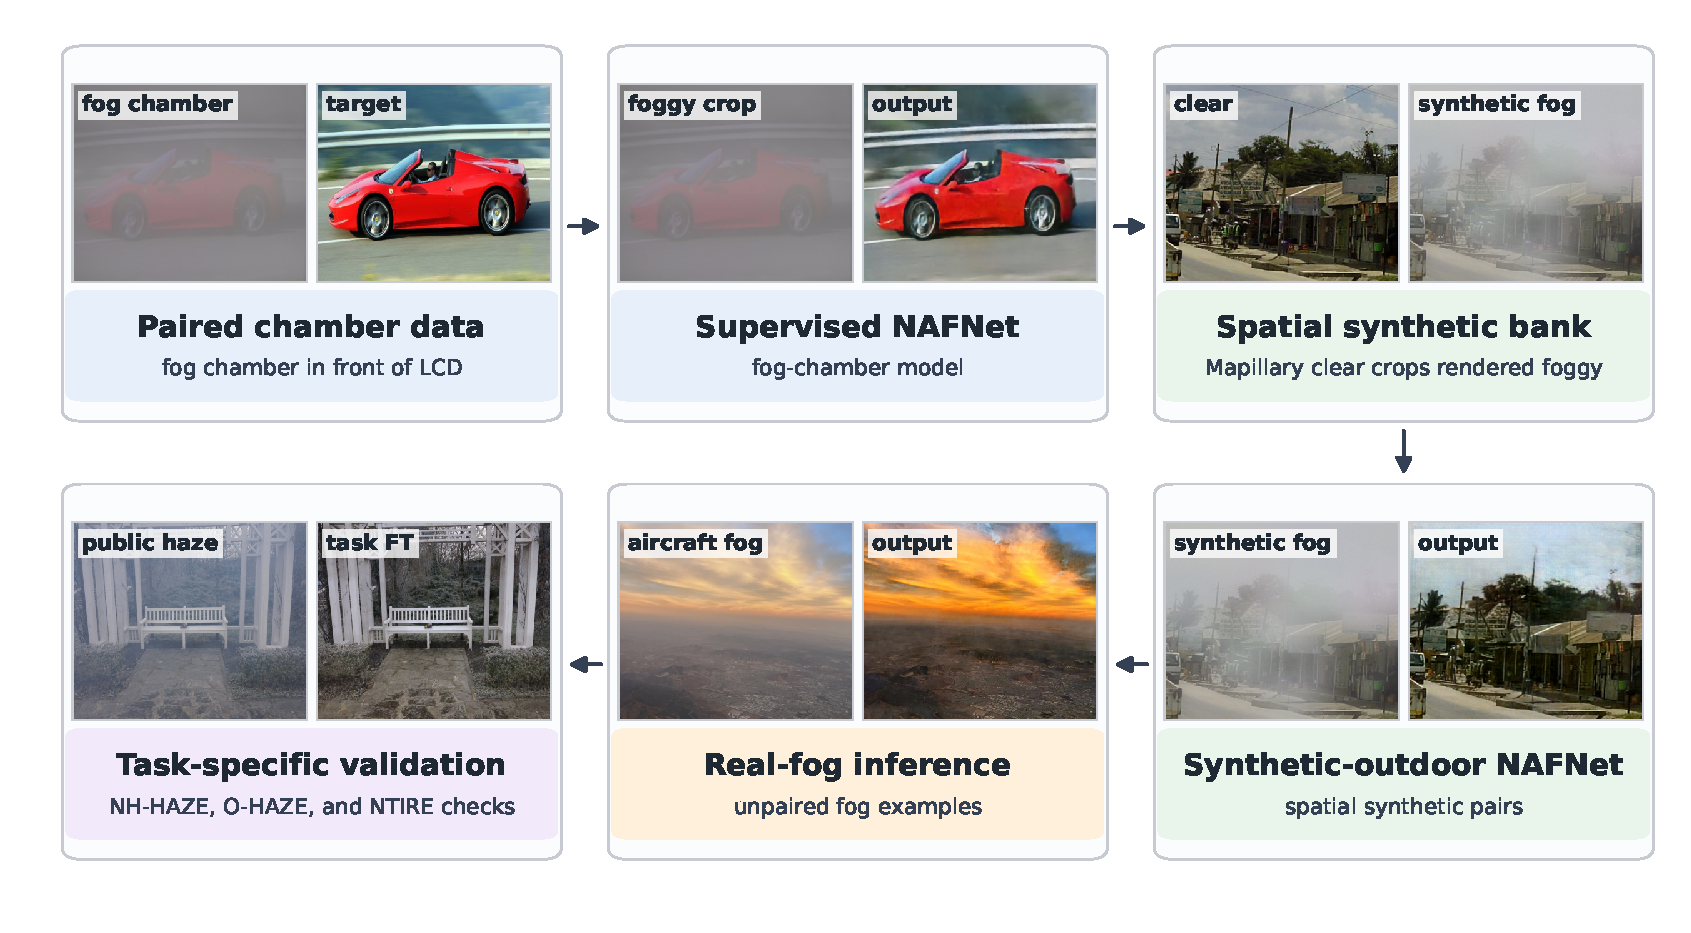
\includegraphics[width=\textwidth]{figures/supplement/figS_transfer_workflow_schematic.pdf}
\caption{Cross-domain transfer workflow. Paired fog-chamber data initialize the supervised NAFNet model. The synthetic fine-tuning branch renders Mapillary clear crops with spatial synthetic fog and fine-tunes against the original clear crops. The resulting model is applied to unpaired real-fog examples and paired public-haze/NTIRE examples without using those paired training splits. Separate NH-HAZE, O-HAZE, and NTIRE NAFNet models provide supervised task-specific checks.}
\label{figS:transfer_workflow_schematic}
\end{figure}
\FloatBarrier

\section{Public Paired Real-Haze Adaptation}

The main manuscript reports the mixed O-HAZE+NH-HAZE adaptation result. O-HAZE contains 45 paired outdoor real-haze images, and NH-HAZE contains 55 paired non-homogeneous real-haze images~\cite{ancuti2018ohaze,ancuti2020nhhaze}. The reported model used only the mixed training policy: O-HAZE images 1--35 and NH-HAZE images 1--45 for training, O-HAZE 36--40 and NH-HAZE 46--50 for validation, and O-HAZE 41--45 plus NH-HAZE 51--55 for testing.

The real-haze fine-tuning run started from the fog-chamber NAFNet model and used random $256 \times 256$ paired hazy/ground-truth crops, L1 reconstruction loss, AdamW, learning rate $10^{-4}$, batch size 4, and early stopping by validation L1. The best validation epoch was 39, and training stopped after epoch 57.

\begin{figure}[htbp]
\centering
\includegraphics[width=\textwidth]{figures/supplement/figS6_external_real_haze_examples.pdf}
\caption{Held-out O-HAZE and NH-HAZE examples showing direct synthetic-fine-tuned transfer and task-specific supervised adaptation. Columns show hazy input, synthetic-fine-tuned NAFNet output with no public-haze training, mixed O-HAZE/NH-HAZE supervised NAFNet output, and paired ground truth. Output stamps on both model columns report PSNR/SSIM against the paired clear target.}
\label{figS:external_real_haze_examples}
\end{figure}

\begin{table}[H]
\centering
\scriptsize
\caption{Supervised mixed real-haze fine-tuning protocol and split audit. Image identity was checked as dataset/image-id pairs across train, validation, and test records.}
\label{tabS:external_training_protocol}
\resizebox{\textwidth}{!}{%
\begin{tabular}{@{}>{\raggedright\arraybackslash}p{0.15\textwidth}>{\raggedright\arraybackslash}p{0.27\textwidth}>{\raggedright\arraybackslash}p{0.23\textwidth}>{\raggedright\arraybackslash}p{0.20\textwidth}cc@{}}
\toprule
\textbf{Model} & \textbf{Training images} & \textbf{Validation images} & \textbf{Test images} & \textbf{Best epoch} & \textbf{Overlap} \\
\midrule
Mixed real-haze fine-tuning & O-HAZE 1--35 + NH-HAZE 1--45 (n=80) & O-HAZE 36--40 + NH-HAZE 46--50 (n=10) & O-HAZE 41--45 + NH-HAZE 51--55 (n=10) & 39 & 0 train/test; 0 validation/test \\
\bottomrule
\end{tabular}
}
\end{table}

\begin{table}[H]
\centering
\small
\caption{Internal test-split metrics for the combined real-haze model. Subset rows are diagnostics of the same model.}
\label{tabS:external_heldout}
\begin{tabular}{@{}>{\raggedright\arraybackslash}p{0.20\textwidth}>{\raggedright\arraybackslash}p{0.32\textwidth}cccc@{}}
\toprule
\textbf{Model} & \textbf{Held-out split} & \textbf{n} & \textbf{MAE} & \textbf{PSNR} & \textbf{SSIM} \\
\midrule
Mixed real haze & O-HAZE 41--45 & 5 & 0.0589 & 22.65 & 0.726 \\
Mixed real haze & NH-HAZE 51--55 & 5 & 0.0894 & 18.77 & 0.640 \\
Mixed real haze & O-HAZE 41--45 + NH-HAZE 51--55 & 10 & 0.0741 & 20.71 & 0.683 \\
\bottomrule
\end{tabular}
\end{table}
\FloatBarrier

 

\subsection{NTIRE 2026 Nighttime Haze Evaluation}

The NTIRE 2026 evaluation used the released nighttime haze training pairs. The available training set contains 25 paired nighttime hazy/ground-truth images. We trained an NTIRE-specific NAFNet from the fog-chamber model using IDs 01--20 for training, IDs 21--23 for validation and model selection, and IDs 24--25 as an internal test split. The best validation epoch was 15, and training stopped after epoch 29. This internal split is useful for checking whether the same backbone adapts to nighttime paired haze, but it is not an official challenge validation/test result because those clear targets are unavailable locally. It therefore does not establish a competition rank.

\begin{table}[H]
\centering
\small
\caption{NTIRE 2026 supervised nighttime-haze result. The held-out IDs 24--25 were not used for training or model selection. Metrics are computed against the released training ground truth.}
\label{tabS:ntire26_supervised}
\begin{tabular}{llcccc}
\toprule
\textbf{Split} & \textbf{Model} & \textbf{n} & \textbf{MAE} & \textbf{PSNR} & \textbf{SSIM} \\
\midrule
Held-out 24--25 & NTIRE NAFNet & 2 & 0.0435 & 24.77 & 0.770 \\
\bottomrule
\end{tabular}
\end{table}
\FloatBarrier

\begin{figure}[htbp]
\centering
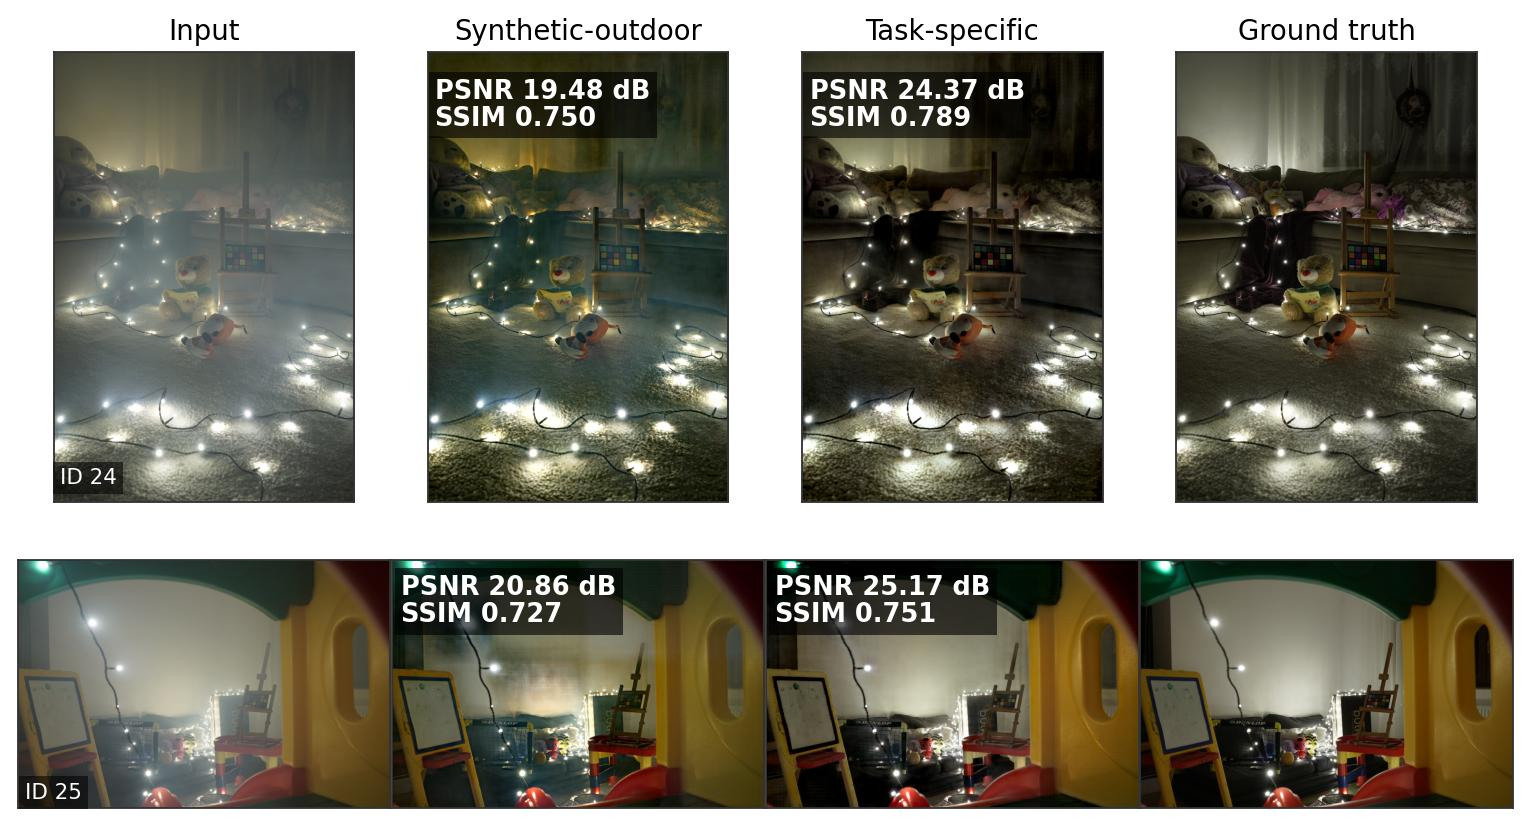
\includegraphics[width=\textwidth]{figures/supplement/figS10_ntire26_localtest_supervised_key_pair.jpg}
\caption{NTIRE 2026 held-out examples 24 and 25 showing direct synthetic-fine-tuned transfer and task-specific supervised adaptation. Columns compare the hazy input, synthetic-fine-tuned NAFNet output with no NTIRE training, NTIRE-specific supervised NAFNet output, and paired ground truth. Output stamps on both model columns report PSNR/SSIM against the released ground truth.}
\label{figS:ntire26_local_examples}
\end{figure}

The mixed real-haze result uses a 10-image internal test split, and the NTIRE 2026 check uses a two-image internal test split from the released training pairs. These checks show that the fog-chamber NAFNet model can be adapted by paired outdoor or nighttime haze supervision, but the training policy, split definition, image size, and reference appearance prevent leaderboard claims.
\FloatBarrier


\section{Fog Density Statistics}

Fog statistics were computed from the 552-image fog-chamber benchmark held-out split and from the clear and light-fog outdoor image sets. Images were converted to numeric pixel values after resizing the longest side to at most 512 pixels for consistent throughput. The dark-channel haze index was the image mean of a 15-pixel minimum-filtered color-channel dark channel, RMS contrast was luminance standard deviation divided by mean luminance, sharpness was the mean finite-difference luminance gradient magnitude, and airlight shift was the change in mean luminance relative to the available clear reference. Chamber statistics used paired fog/clear archive images, so contrast, luminance-standard-deviation, and gradient attenuation were reported as fog-over-clear ratios. The outdoor clear and light-fog captures are independent groups, so outdoor attenuation was reported only as a group-level light-fog/clear ratio.

\begin{figure}[htbp]
\centering
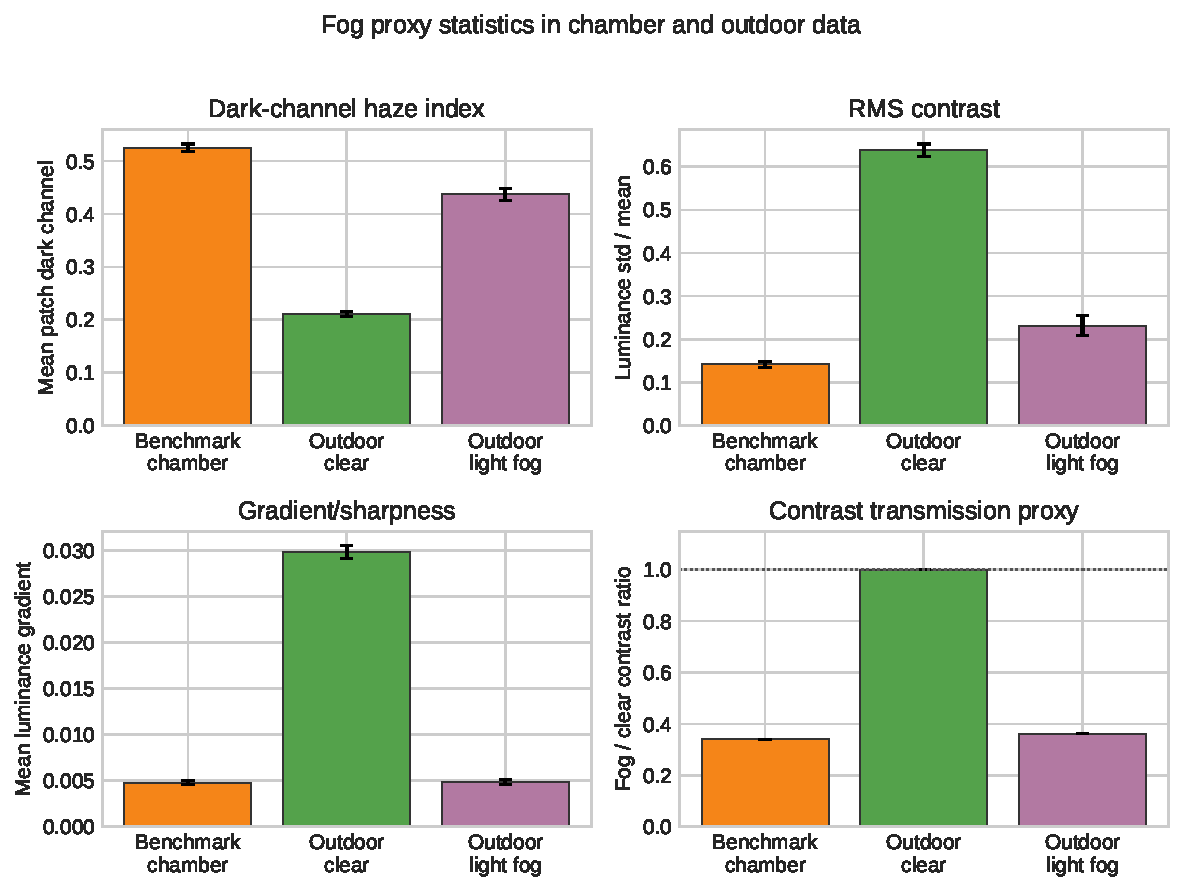
\includegraphics[width=0.95\textwidth]{figures/supplement/figS4_fog_density_proxy_statistics.pdf}
\caption{Simple fog statistics for the chamber and outdoor data. The chamber condition uses paired fog/clear archive references; the outdoor light-fog condition uses the outdoor clear group as an independent reference. Error bars show 95\% confidence intervals for absolute per-image metrics.}
\label{figS:fog_density_proxy}
\end{figure}

\begin{table}[htbp]
\centering
\small
\caption{Fog statistics comparing chamber and outdoor data. Ratios are fog/reference values, where the reference is the paired clear archive image for chamber data and the outdoor clear group mean for outdoor light fog.}
\label{tabS:fog_density_proxy}
\begin{tabular}{lccccc}
\toprule
\textbf{Condition} & \textbf{n} & \textbf{Dark channel} & \textbf{RMS contrast} & \textbf{Grad. mag.} & \textbf{Contrast ratio} \\
\midrule
Benchmark chamber & 552 & 0.526 & 0.142 & 0.00478 & 0.340 \\
Outdoor clear & 430 & 0.211 & 0.639 & 0.02988 & 1.000 \\
Outdoor light fog & 84 & 0.437 & 0.232 & 0.00483 & 0.363 \\
\bottomrule
\end{tabular}
\end{table}

The statistics separated clear and fogged imagery in both acquisition regimes. For the benchmark chamber data, RMS contrast was 0.340 of the paired clear reference and mean gradient was 0.181 of clear. Outdoor light fog also moved in the expected direction relative to outdoor clear: dark-channel haze index increased from 0.211 to 0.437, RMS contrast fell to 0.363 of the clear outdoor group, and mean gradient fell to 0.162 of clear. Thus the statistics support a defensible relative fog-index comparison across chamber and free-space data, but they do not establish physical fog density without distance and calibration.

\section{Image-Domain Power-Spectral Analysis}
\label{secS:psd_image_domain}

We used the paired chamber data to quantify how fog changes spatial-frequency content in the recorded images. For each held-out pair, the foggy chamber capture and the corresponding archive image displayed on the screen were converted to luminance, resized to $512 \times 512$, mean-subtracted, Hann-windowed, Fourier transformed, and radially averaged into 96 spatial-frequency bins. We then computed the per-pair radial power-spectral-density (PSD) ratio,
\begin{equation}
R_{\mathrm{PSD}}(f) =
\frac{P_{\mathrm{fog}}(f)}
     {P_{\mathrm{archive}}(f)} ,
\label{eqS:psd_ratio}
\end{equation}
where $P_{\mathrm{fog}}(f)$ is the foggy camera-capture PSD and $P_{\mathrm{archive}}(f)$ is the PSD of the displayed archive image. The deterministic every-tenth held-out split gave $n=552$ pairs.

This is an image-domain degradation measurement, not a physical transmission spectrum of the fog. The ratio includes the display, chamber, fog, lens, sensor, exposure, camera processing, and resizing pipeline. It is therefore used only to summarize loss of recorded spatial detail.

The median paired PSD ratio was 0.0322 (95\% bootstrap CI 0.0294--0.0372) over low spatial frequencies, 0.01--0.05 cycles/pixel, and 0.0036 (95\% CI 0.0033--0.0041) over higher spatial frequencies, 0.15--0.24 cycles/pixel. Thus high-frequency power was retained 8.9$\times$ less than low-frequency power in the paired image-domain measurement. This frequency-domain result supports the Laplacian-retention analysis in the main text: foggy captures lose fine spatial structure disproportionately, making high-texture scenes harder to restore.

\begin{figure}[htbp]
\centering
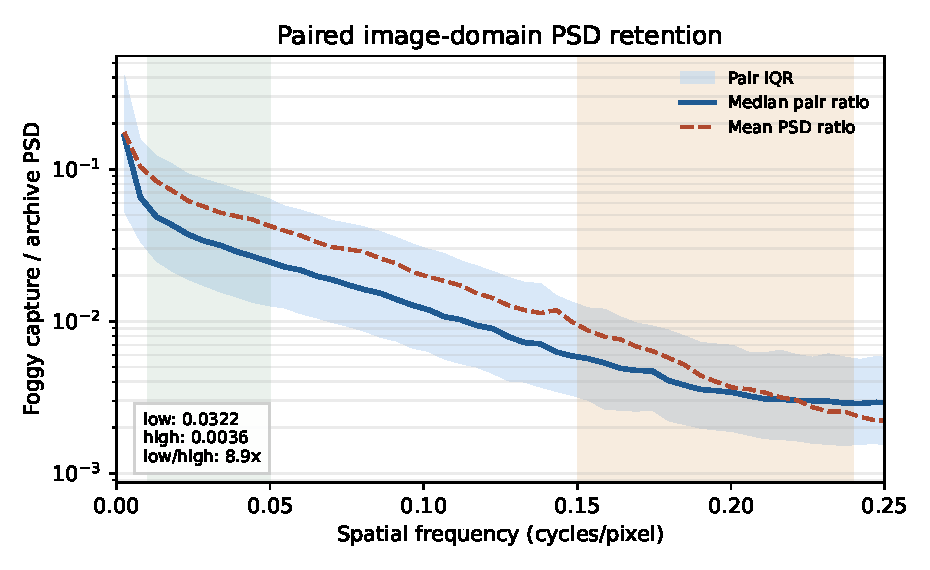
\includegraphics[width=0.85\textwidth]{figures/supplement/paired_psd_retention.pdf}
\caption{Paired image-domain power-spectral-density retention for the held-out chamber split. The solid line shows the median foggy-capture/archive PSD ratio across image pairs; the shaded band shows the interquartile range. The dashed line shows the ratio of mean foggy and archive PSDs. Green and orange bands mark the low- and high-frequency ranges summarized in the text.}
\label{figS:paired_psd_retention}
\end{figure}
\FloatBarrier

\section{Paired Structure-Loss Metrics and Restoration Difficulty}
\label{secS:paired_structure_metrics}

We used the 552-image fog-chamber benchmark held-out split to ask whether simple image statistics tracked image-level NAFNet restoration quality. Each foggy image was paired with its aligned clear archive target. We compared foggy-image-only haze proxies with paired structure-loss metrics computed from the fog/clear pair.

The strongest single paired statistic was the mean absolute Laplacian-response ratio,
\begin{equation}
r_{\nabla^2} =
\frac{\mathrm{mean}\left(\left|\nabla^2 I_{\mathrm{fog}}\right|\right)}
{\mathrm{mean}\left(\left|\nabla^2 I_{\mathrm{clear}}\right|\right)} ,
\label{eqS:laplacian_ratio}
\end{equation}
where $I_{\mathrm{fog}}$ and $I_{\mathrm{clear}}$ are luminance images. This ratio measures how much fine spatial structure remains in the foggy image relative to the aligned clear target. It had Spearman correlation $\rho=0.632$ with per-image NAFNet PSNR. By comparison, the strongest foggy-image-only statistic in this subset, the 90th percentile dark-channel response, reached $\rho=0.399$.

We also evaluated the same mean-absolute Laplacian ratio using wider finite-difference steps, where step~1 is the nearest-neighbor five-point Laplacian and larger steps compare pixels separated by 3, 8, or 12 pixels. Correlation with NAFNet PSNR decreased as the step widened ($\rho=0.542$ at step~3 and $0.417$ at step~8), indicating that the most predictive signal was fine-scale structure retention rather than broader luminance variation. A separate PSD fit summarized each fog/clear pair by a single equivalent Gaussian-PSF width, but this scalar blur width was only a weak predictor of restoration quality ($\rho=-0.206$), so we treat it as a diagnostic rather than the primary difficulty metric.

\begin{figure}[htbp]
\centering
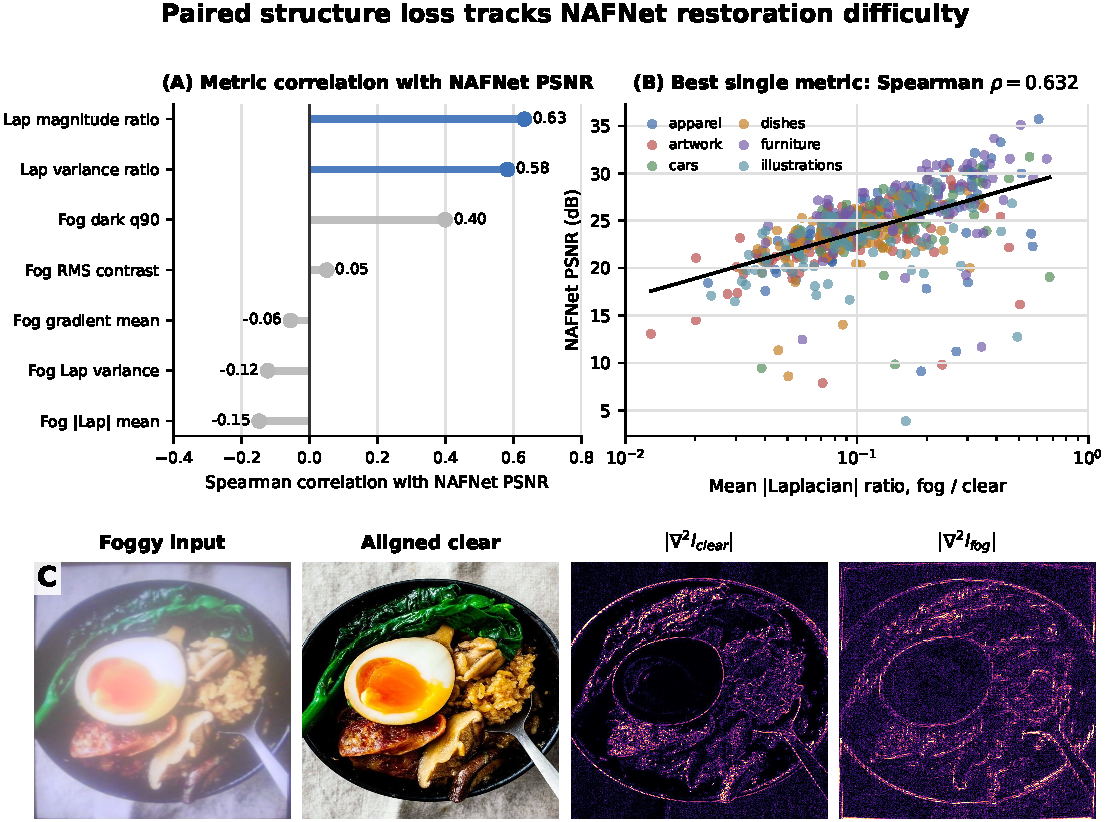
\includegraphics[width=\textwidth]{figures/supplement/figS_paired_structure_loss_metric.pdf}
\caption{Paired structure-loss metrics track NAFNet restoration difficulty on the fog-chamber held-out split. (A) Signed Spearman correlations between selected paired and foggy-only image statistics and per-image NAFNet PSNR, with $\rho$ values labeled next to each point. (B) Per-image NAFNet PSNR plotted against the strongest single metric, the scalar fog/clear mean absolute Laplacian-response ratio. Points are colored by archive category, and the black line shows a fit versus $\log_{10}$ of the metric. (C) Example showing the foggy input, aligned clear target, and independently contrast-scaled absolute Laplacian-response maps for clear and foggy images.}
\label{figS:paired_structure_metric}
\end{figure}

The statistic is a scalar ratio of two full-image averages, not the average of a pixelwise ratio map. Thus, locations with larger absolute Laplacian response contribute more to the numerator and denominator, whereas flat regions contribute little. These results suggest that image-level restoration difficulty is not captured by foggy-image haze proxies alone. Paired structure loss, especially loss of Laplacian response, better tracks NAFNet PSNR because it measures how much high-frequency scene detail survives the fog-imaging process. The statistic is a relative restoration-difficulty index, not a calibrated physical fog-density measurement.

\begin{table}[htbp]
\centering
\small
\caption{No-reference NIQE scores for representative out-of-domain examples. Lower NIQE is better. The fog-machine and aircraft-window rows use the synthetic-fine-tuned output images. The O-HAZE and NH-HAZE rows use the mixed real-haze supervised output images, and the NTIRE row uses the NTIRE-specific supervised output images.}
\label{tabS:niqe_transfer}
\begin{tabular}{lrrrr}
\toprule
\textbf{Dataset} & \textbf{n} & \textbf{Input NIQE} & \textbf{Output NIQE} & \textbf{NIQE decrease} \\
\midrule
Aircraft-window & 43 & 6.22 & 4.97 & 1.25 \\
Fog-machine free fog & 99 & 5.05 & 3.61 & 1.44 \\
O-HAZE & 5 & 4.15 & 4.03 & 0.12 \\
NH-HAZE & 5 & 2.83 & 3.55 & -0.71 \\
NTIRE 2026 nighttime haze & 2 & 4.94 & 4.84 & 0.10 \\
\bottomrule
\end{tabular}
\end{table}
\FloatBarrier

\bibliography{defogging_supplement_refs}

\end{document}
